\section{Matrix}
\subsection{矩阵基础}

TikZ 中的矩阵类似于 \LaTeX 中的表格,矩阵中各元素的控制则与 Node 十分相似,因为 Matrix 本质上就是 Node 的集合。

\subsubsection{节点形式的矩阵}

在 Node 中可以使用 matrix 选项,指定某个节点为矩阵。在内部可以使用 \LaTeX 表格的语法。

\begin{figure}[H]
    \centering
    \begin{minipage}{0.35\linewidth}
        \centering
        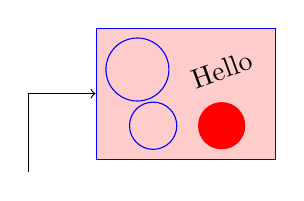
\begin{tikzpicture}[scale = 1]
            \node [matrix,fill=red!20,draw=blue] (my matrix) at (2,1) {
                \draw (0,0) circle (4mm); & \node [rotate=20] {Hello}; \\
                \draw (0.2,0) circle (3mm); & \fill[red] (0,0) circle (3mm); \\
            };
            \draw [->] (0,0) |- (my matrix.west);
        \end{tikzpicture}
    \end{minipage}
    \begin{minipage}{0.55\linewidth}
        \begin{lstlisting}[style = latex-side]
    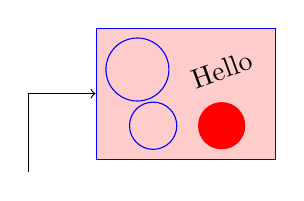
\begin{tikzpicture}[scale = 1]
        \node [matrix,fill=red!20,draw=blue] (my matrix) at (2,1) {
            \draw (0,0) circle (4mm); & \node [rotate=20] {Hello}; \\
            \draw (0.2,0) circle (3mm); & \fill[red] (0,0) circle (3mm); \\
        };
        \draw [->] (0,0) |- (my matrix.west);
    \end{tikzpicture}
        \end{lstlisting}
    \end{minipage}
    \caption{Matrix:节点形式的矩阵}
\end{figure}

\textbackslash every matrix 控制矩阵样式,这将同时控制矩阵内部图形的样式 

\textbackslash every outer matrix 仅控制矩阵框样式。

\textbackslash matrix 是 \textbackslash path node [matrix] 的简写。 

尽管矩阵是由节点引申来的,但有些修饰无法使用:

\begin{itemize}[itemindent=2em]
    \item rotation 和 scale 对节点框无效。
    \item matrix 节点无法被拆分。
    \item 所有以 text- 开头的修饰均无效。
    \item matrix 在放置在路径上时,会出现许多错误。
\end{itemize}


\subsubsection{矩阵位置}

可以使用 matrix anchor = <anchor> 调整矩阵位置,注意 anchor = <anchor> 调整的是矩阵内单元格的对齐方式

\begin{figure}[H]
    \centering
    \begin{minipage}{0.35\linewidth}
        \centering
        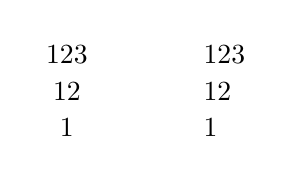
\begin{tikzpicture}[scale = 1]
            \matrix [matrix anchor=west] at (0,0) {
                \node {123}; \\ % still center anchor
                \node {12}; \\
                \node {1}; \\
            };
            \matrix [anchor=west] at (2,0) {
                \node {123}; \\ % inherited west anchor
                \node {12}; \\
                \node {1}; \\
            };
        \end{tikzpicture}
    \end{minipage}
    \begin{minipage}{0.55\linewidth}
        \begin{lstlisting}[style = latex-side]
    \begin{tikzpicture}[scale = 1]
        \matrix [matrix anchor=west] at (0,0) {
            \node {123}; \\ % still center anchor
            \node {12}; \\
            \node {1}; \\
        };
        \matrix [anchor=west] at (0,-2) {
            ...
        };
    \end{tikzpicture}
        \end{lstlisting}
    \end{minipage}
    \caption{Matrix:矩阵位置}
\end{figure}


\subsubsection{单元格}

矩阵内部的每个元素均可视为一个单元格,使用 \textbackslash\textbackslash 划分行,使用 \& 划分列。矩阵每行/列的宽度与高度均取决于数值最大的单元格。

\begin{figure}[H]
    \centering
    \begin{minipage}{0.35\linewidth}
        \centering
        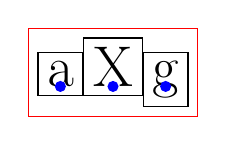
\begin{tikzpicture}[every node/.style = {draw = black,anchor = base,font = \huge}]
            \matrix [draw = red]{
                \node {a}; \fill [blue] (0,0) circle (2pt); &
                \node {X}; \fill [blue] (0,0) circle (2pt); &
                \node {g}; \fill [blue] (0,0) circle (2pt); \\
            };
        \end{tikzpicture}
    \end{minipage}
    \begin{minipage}{0.55\linewidth}
        \begin{lstlisting}[style = latex-side]
    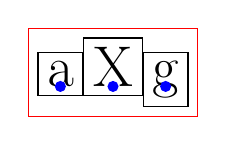
\begin{tikzpicture}[every node/.style = {draw = black,anchor = base,font = \huge}]
        \matrix [draw = red]{
            \node {a}; \fill [blue] (0,0) circle (2pt); &
            \node {X}; \fill [blue] (0,0) circle (2pt); &
            \node {g}; \fill [blue] (0,0) circle (2pt); \\
        };
    \end{tikzpicture}
        \end{lstlisting}
    \end{minipage}
    \caption{Matrix:单元格}
\end{figure}

Matrix 中每行的高度与深度均由行本身决定,默认情况下,行之间间隙为0,可以使用 row sep 指定间隙。

\begin{figure}[H]
    \centering
    \begin{minipage}{0.35\linewidth}
        \centering
        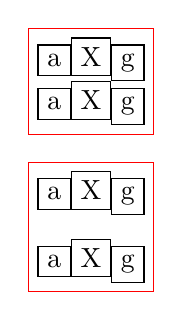
\begin{tikzpicture}[every node/.style = {draw = black,anchor = base}]
            \matrix [draw = red]{
                \node {a}; & \node {X}; & \node {g};  \\
                \node {a}; & \node {X}; & \node {g};  \\
            };
            \matrix [draw = red,row sep = 3mm] at (0,-2){
                \node {a}; & \node {X}; & \node {g};  \\
                \node {a}; & \node {X}; & \node {g};  \\
            };
        \end{tikzpicture}
    \end{minipage}
    \begin{minipage}{0.55\linewidth}
        \begin{lstlisting}[style = latex-side]
    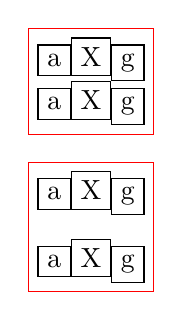
\begin{tikzpicture}[every node/.style = {draw = black,anchor = base}]
        \matrix [draw = red]{
            \node {a}; & \node {X}; & \node {g};  \\
            \node {a}; & \node {X}; & \node {g};  \\
        };
        \matrix [draw = red,row sep = 3mm] at (0,-2){
            \node {a}; & \node {X}; & \node {g};  \\
            \node {a}; & \node {X}; & \node {g};  \\
        };
    \end{tikzpicture}
        \end{lstlisting}
    \end{minipage}
    \caption{Matrix:行间隙}
\end{figure}

矩阵的列与行一样,列宽取决于每列的最大宽度,默认列之间间隙为0,可以通过 column sep 调整列宽。

\begin{figure}[H]
    \centering
    \begin{minipage}{0.35\linewidth}
        \centering
        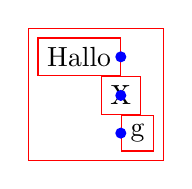
\begin{tikzpicture}[every node/.style={draw}]
            \matrix [draw=red]{
                \node[left] {Hallo};    \fill[blue] (0,0) circle (2pt); \\
                \node {X};              \fill[blue] (0,0) circle (2pt); \\
                \node[right] {g};       \fill[blue] (0,0) circle (2pt); \\
            };
        \end{tikzpicture}
    \end{minipage}
    \begin{minipage}{0.55\linewidth}
        \begin{lstlisting}[style = latex-side]
    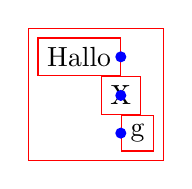
\begin{tikzpicture}[every node/.style={draw}]
        \matrix [draw=red]{
            \node[left] {Hallo};    \fill[blue] (0,0) circle (2pt); \\
            \node {X};              \fill[blue] (0,0) circle (2pt); \\
            \node[right] {g};       \fill[blue] (0,0) circle (2pt); \\
        };
    \end{tikzpicture}
        \end{lstlisting}
    \end{minipage}
    \caption{Matrix:列宽}
\end{figure}

\begin{figure}[H]
    \centering
    \begin{minipage}{0.35\linewidth}
        \centering
        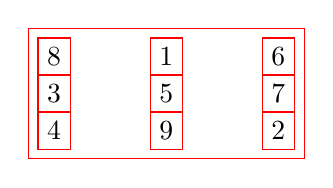
\begin{tikzpicture}[every node/.style={draw}]
            \matrix [draw=red,column sep=1cm]{
                \node {8}; & \node{1}; & \node {6}; \\
                \node {3}; & \node{5}; & \node {7}; \\
                \node {4}; & \node{9}; & \node {2}; \\
            };
        \end{tikzpicture}
    \end{minipage}
    \begin{minipage}{0.55\linewidth}
        \begin{lstlisting}[style = latex-side]
    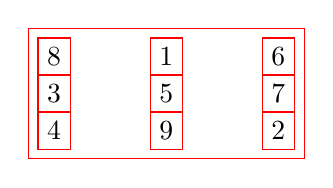
\begin{tikzpicture}[every node/.style={draw}]
        \matrix [draw=red,column sep=1cm]{
            \node {8}; & \node{1}; & \node {6}; \\
            \node {3}; & \node{5}; & \node {7}; \\
            \node {4}; & \node{9}; & \node {2}; \\
        };
    \end{tikzpicture}
        \end{lstlisting}
    \end{minipage}
    \caption{Matrix:列间隙}
\end{figure}

\subsection{矩阵样式}
\subsubsection{矩阵间距}

控制矩阵间隔有两种方式:1.通过 \textbf{row sep} 或 \textbf{column sep} 控制所有行列的宽度。2. 通过 \textbackslash\textbackslash 或 \& 精确控制某一行/列。

\begin{itemize}
    \item 列间距 \\
    列间距:[column sep = <spacing list>]:用来控制默认列间距,值可以是正数或负数。\\
    这里的 <spacing list> 类似于 <dimension>

    \begin{figure}[H]
        \centering
        \begin{minipage}{0.35\linewidth}
            \centering
            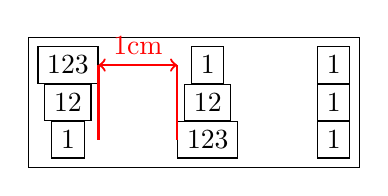
\begin{tikzpicture}
                \matrix [draw,column sep = 1cm,nodes = draw]{
                    \node(a) {123}; & \node (b) {1};    & \node {1}; \\
                    \node {12};     & \node {12};       & \node {1}; \\
                    \node(c) {1};   & \node (d) {123};  & \node {1}; \\
                };
                \draw [red,thick] (a.east) -- (a.east |- c)
                                    (d.west) -- (d.west |- b);
                \draw [<->,red,thick] (a.east) -- (d.west |- b)
                                    node [above,midway] {1cm};
            \end{tikzpicture}
        \end{minipage}
        \begin{minipage}{0.55\linewidth}
            \begin{lstlisting}[style = latex-side]
    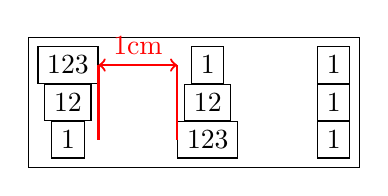
\begin{tikzpicture}
        \matrix [draw,column sep = 1cm,nodes = draw]{
            \node(a) {123}; & \node (b) {1};    & \node {1}; \\
            \node {12};     & \node {12};       & \node {1}; \\
            \node(c) {1};   & \node (d) {123};  & \node {1}; \\
        };
        \draw [red,thick] (a.east) -- (a.east |- c)
                            (d.west) -- (d.west |- b);
        \draw [<->,red,thick] (a.east) -- (d.west |- b)
                            node [above,midway] {1cm};
    \end{tikzpicture}
            \end{lstlisting}
        \end{minipage}
        \caption{Matrix:column sep}
    \end{figure}

间距默认为单元格的边界,我们也可以指定从单元格原点开始计算。

\begin{figure}[H]
    \centering
    \begin{minipage}{0.35\linewidth}
        \centering
        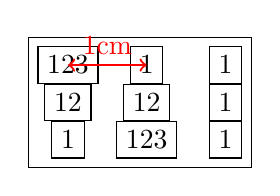
\begin{tikzpicture}
            \matrix [draw,column sep={1cm,between origins},nodes=draw]{
                \node(a) {123}; & \node (b) {1}; & \node {1}; \\
                \node {12}; & \node {12}; & \node {1}; \\
                \node {1}; & \node {123}; & \node {1}; \\
            };
            \draw [<->,red,thick] (a.center) -- (b.center) node [above,midway] {1cm};
        \end{tikzpicture}
    \end{minipage}
    \begin{minipage}{0.55\linewidth}
        \begin{lstlisting}[style = latex-side]
    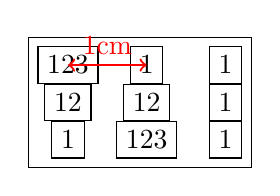
\begin{tikzpicture}
        \matrix [draw,column sep={1cm,between origins},nodes=draw]{
            \node(a) {123}; & \node (b) {1}; & \node {1}; \\
            \node {12}; & \node {12}; & \node {1}; \\
            \node {1}; & \node {123}; & \node {1}; \\
        };
        \draw [<->,red,thick] (a.center) -- (b.center) node [above,midway] {1cm};
    \end{tikzpicture}
        \end{lstlisting}
    \end{minipage}
    \caption{Matrix:origin 的 column sep}
\end{figure}

\item 行间距\\
行间距:[row sep = <spacing list>]:控制各行之间间距,用法和列间距相同

\begin{figure}[H]
    \centering
    \begin{minipage}{0.35\linewidth}
        \centering
        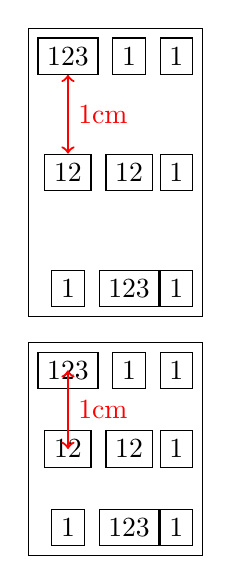
\begin{tikzpicture}[scale = 1]
            \matrix [draw,row sep=1cm,nodes=draw]{
                \node (a) {123}; & \node {1}; & \node {1}; \\
                \node (b) {12}; & \node {12}; & \node {1}; \\
                \node {1}; & \node {123}; & \node {1}; \\
            };
            \draw [<->,red,thick] (a.south) -- (b.north) node [right,midway] {1cm};

            \matrix [draw,row sep={1cm,between origins},nodes=draw] at (0,-10em){
                \node (a) {123}; & \node {1}; & \node {1}; \\
                \node (b) {12}; & \node {12}; & \node {1}; \\
                \node {1}; & \node {123}; & \node {1}; \\
            };
            \draw [<->,red,thick] (a.center) -- (b.center) node [right,midway] {1cm};
        \end{tikzpicture}
    \end{minipage}
    \begin{minipage}{0.55\linewidth}
        \begin{lstlisting}[style = latex-side]
    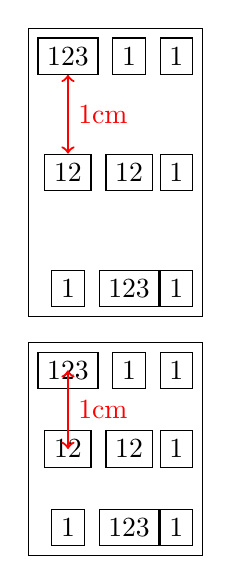
\begin{tikzpicture}[scale = 1]
        \matrix [draw,row sep=1cm,nodes=draw]{
            \node (a) {123}; & \node {1}; & \node {1}; \\
            \node (b) {12}; & \node {12}; & \node {1}; \\
            \node {1}; & \node {123}; & \node {1}; \\
        };
        \draw [<->,red,thick] (a.south) -- (b.north) node [right,midway] {1cm};
        \matrix [draw,row sep={1cm,between origins},nodes=draw] at (0,-10em){
            \node (a) {123}; & \node {1}; & \node {1}; \\
            \node (b) {12}; & \node {12}; & \node {1}; \\
            \node {1}; & \node {123}; & \node {1}; \\
        };
        \draw [<->,red,thick] (a.center) -- (b.center) node [right,midway] {1cm};
    \end{tikzpicture}
        \end{lstlisting}
    \end{minipage}
    \caption{Matrix:row sep}
\end{figure}

\item 精确间距 \\
上述的控制方法只能设置整体的默认间距,精确到某行/列则需要在分隔符中设定距离。

\begin{figure}[H]
    \centering
    \begin{minipage}{0.35\linewidth}
        \centering
        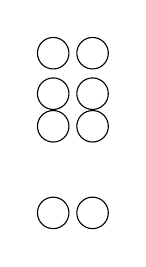
\begin{tikzpicture}[scale = 1]
            \matrix [row sep=1mm]{
                \draw (0,0) circle (2mm); &[0.5cm,between origins] \draw (0,0) circle (2mm); \\
                \draw (0,0) circle (2mm); & \draw (0,0) circle (2mm); \\[-1mm]
                \draw (0,0) coordinate (a) circle (2mm); &
                \draw (0,0) circle (2mm); \\[1cm,between origins]
                \draw (0,0) coordinate (b) circle (2mm); &
                \draw (0,0) circle (2mm); \\
            };
        \end{tikzpicture}
    \end{minipage}
    \begin{minipage}{0.55\linewidth}
        \begin{lstlisting}[style = latex-side]
    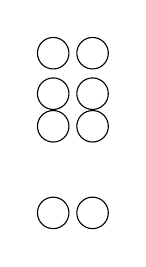
\begin{tikzpicture}[scale = 1]
        \matrix [row sep=1mm]{
            \draw (0,0) circle (2mm); &[0.5cm,between origins] \draw (0,0) circle (2mm); \\
            \draw (0,0) circle (2mm); & \draw (0,0) circle (2mm); \\[-1mm]
            \draw (0,0) coordinate (a) circle (2mm); &
            \draw (0,0) circle (2mm); \\[1cm,between origins]
            \draw (0,0) coordinate (b) circle (2mm); &
            \draw (0,0) circle (2mm); \\
        };
    \end{tikzpicture}
        \end{lstlisting}
    \end{minipage}
    \caption{Matrix:}
\end{figure}

\end{itemize}

\subsubsection{单元格样式}

矩阵往往包含多个单元格,逐一控制往往不太现实,TikZ 提供了许多批量控制的修饰。

\begin{itemize}
    \item every cell = {<row>}{<column>}: 设置矩阵行列数量
    \item cells = <options>: 设置每个单元格的样式,等效于 every cell/.append style = <options>
    \item nodes = <options>: 设置每个节点的样式
    \begin{figure}[H]
        \centering
        \begin{minipage}{0.35\linewidth}
            \centering
            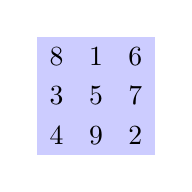
\begin{tikzpicture}[scale = 1]
                \matrix [nodes={fill=blue!20,minimum size=5mm}]{
                    \node {8}; & \node{1}; & \node {6}; \\
                    \node {3}; & \node{5}; & \node {7}; \\
                    \node {4}; & \node{9}; & \node {2}; \\
                };
            \end{tikzpicture}
        \end{minipage}
        \begin{minipage}{0.55\linewidth}
            \begin{lstlisting}[style = latex-side]
    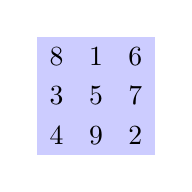
\begin{tikzpicture}[scale = 1]
        \matrix [nodes={fill=blue!20,minimum size=5mm}]{
            \node {8}; & \node{1}; & \node {6}; \\
            \node {3}; & \node{5}; & \node {7}; \\
            \node {4}; & \node{9}; & \node {2}; \\
        };
    \end{tikzpicture}
            \end{lstlisting}
        \end{minipage}
        \caption{Matrix:节点样式}
    \end{figure}

    \item column <number>: 设置<number>列的样式
    \item every odd column: 设置奇数列样式
    \item every even column: 设置偶数列样式
    \item row <number>: 设置<number>行的样式
    \item every odd row: 设置奇数行样式
    \item every even row: 设置偶数行样式
    \item row <number> column <number>: 设置对应行列下某个单元格的样式
    \begin{figure}[H]
        \centering
        \begin{minipage}{0.35\linewidth}
            \centering
            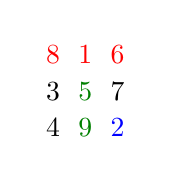
\begin{tikzpicture} [row 1/.style={red}, column 2/.style={green!50!black}, row 3 column 3/.style={blue}]
                \matrix{
                    \node {8}; & \node{1}; & \node {6}; \\
                    \node {3}; & \node{5}; & \node {7}; \\
                    \node {4}; & \node{9}; & \node {2}; \\
                };
            \end{tikzpicture}
        \end{minipage}
        \begin{minipage}{0.55\linewidth}
            \begin{lstlisting}[style = latex-side]
    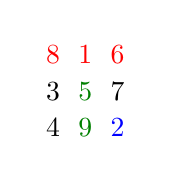
\begin{tikzpicture} [row 1/.style={red}, column 2/.style={green!50!black}, row 3 column 3/.style={blue}]
        \matrix{
            \node {8}; & \node{1}; & \node {6}; \\
            \node {3}; & \node{5}; & \node {7}; \\
            \node {4}; & \node{9}; & \node {2}; \\
        };
    \end{tikzpicture}
            \end{lstlisting}
        \end{minipage}
        \caption{Matrix:单元格样式}
    \end{figure}

    \begin{figure}[H]
        \centering
        \begin{minipage}{0.35\linewidth}
            \centering
            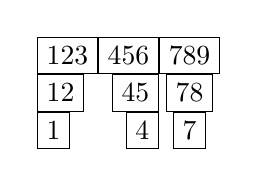
\begin{tikzpicture} [column 1/.style={anchor=base west}, column 2/.style={anchor=base east}, column 3/.style={anchor=base}]
                \matrix[nodes = draw]{
                    \node {123}; & \node{456}; & \node {789}; \\
                    \node {12}; & \node{45}; & \node {78}; \\
                    \node {1}; & \node{4}; & \node {7}; \\
                };
            \end{tikzpicture}
        \end{minipage}
        \begin{minipage}{0.55\linewidth}
            \begin{lstlisting}[style = latex-side]
    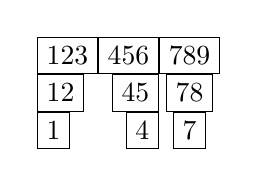
\begin{tikzpicture} [column 1/.style={anchor=base west}, column 2/.style={anchor=base east}, column 3/.style={anchor=base}]
        \matrix[nodes = draw]{
            \node {123}; & \node{456}; & \node {789}; \\
            \node {12}; & \node{45}; & \node {78}; \\
            \node {1}; & \node{4}; & \node {7}; \\
        };
    \end{tikzpicture}
            \end{lstlisting}
        \end{minipage}
        \caption{Matrix:单元格对齐}
    \end{figure}

    \item execute at begin cell = <code>: 在每行非空的第一个单元格执行
    \item execute at end cell = <code>: 在每行非空的最后一个单元格执行
    \item execute at empty cell = <code>: 在每行空的单元格执行
    
    \begin{figure}[H]
        \centering
        \begin{minipage}{0.35\linewidth}
            \centering
            \begin{tikzpicture}[matrix of nodes/.style={
                    execute at begin cell=\node\bgroup,
                    execute at end cell=\egroup;,%
                    execute at empty cell=\node{--};%
                }]
                \matrix [matrix of nodes]{
                    8 & 1 & \\
                    3 & & 7 \\
                    & & 2 \\
                };
            \end{tikzpicture}
        \end{minipage}
        \begin{minipage}{0.55\linewidth}
            \begin{lstlisting}[style = latex-side]
    \begin{tikzpicture}[matrix of nodes/.style={
        execute at begin cell=\node\bgroup,
        execute at end cell=\egroup;,%
        execute at empty cell=\node{--};%
        }]
        \matrix [matrix of nodes]{
            8 & 1 & \\
            3 & & 7 \\
            & & 2 \\
        };
    \end{tikzpicture}
            \end{lstlisting}
        \end{minipage}
        \caption{}
    \end{figure}

\end{itemize}

\subsection{例子}

\begin{figure}[H]
    \centering
    \begin{minipage}{0.35\linewidth}
        \centering
        \begin{tikzpicture}[scale = 1]
            \matrix [matrix of math nodes,row sep=1cm] {
                |(U)| U &[2mm]                  &[8mm] \\
                        & |(XZY)| X \times_Z Y  & |(X)| X \\
                        & |(Y)| Y               & |(Z)| Z \\
            };
            \begin{scope}[every node/.style={midway,auto,font=\scriptsize}]
                \draw [double, dashed] (U) -- node {$x$} (X);
                \draw   (X) -- node {$p$} (X -| XZY.east)
                        (X) -- node {$f$} (Z)
                        -- node {$g$} (Y)
                        -- node {$q$} (XZY)
                        -- node {$y$} (U);
            \end{scope}
        \end{tikzpicture}
    \end{minipage}
    \begin{minipage}{0.55\linewidth}
        \begin{lstlisting}[style = latex-side]
    \begin{tikzpicture}[scale = 1]
        \matrix [matrix of math nodes,row sep=1cm] {
            |(U)| U &[2mm]                  &[8mm] \\
                    & |(XZY)| X \times_Z Y  & |(X)| X \\
                    & |(Y)| Y               & |(Z)| Z \\
        };
        \begin{scope}[every node/.style={midway,auto,font=\scriptsize}]
            \draw [double, dashed] (U) -- node {$x$} (X);
            \draw   (X) -- node {$p$} (X -| XZY.east)
                    (X) -- node {$f$} (Z)
                    -- node {$g$} (Y)
                    -- node {$q$} (XZY)
                    -- node {$y$} (U);
        \end{scope}
    \end{tikzpicture}
        \end{lstlisting}
    \end{minipage}
    \caption{Matrix:例子1}
\end{figure}

\begin{figure}[H]
    \centering
    \begin{minipage}{0.35\linewidth}
        \centering
        \begin{tikzpicture}[>=stealth,->,shorten >=2pt,looseness=.5,auto]
            \matrix [matrix of math nodes,column sep={2cm,between origins},
                row sep={3cm,between origins},nodes={circle, draw, minimum size=7.5mm}]
            {
                        & |(A)| A &         \\
                |(B)| B & |(E)| E & |(C)| C \\
                        & |(D)| D           \\
            };
            \begin{scope}[every node/.style={font=\small\itshape}]
                \draw (A) to [bend left] node [midway] {g} (B);
                \draw (B) to [bend left] node [midway] {f} (A);
                \draw (D) -- node [midway] {c} (B);
                \draw (E) -- node [midway] {b} (B);
                \draw (E) -- node [near end] {a} (C);
                \draw [-,line width=8pt,draw=white]
                    (D) to [bend right, looseness=1] (A);
                \draw (D) to [bend right, looseness=1]
                    node [near start] {b} node [near end] {e} (A);
            \end{scope}
        \end{tikzpicture}
    \end{minipage}
    \begin{minipage}{0.55\linewidth}
        \begin{lstlisting}[style = latex-side]
    \begin{tikzpicture}[>=stealth,->,shorten >=2pt,looseness=.5,auto]
        \matrix [matrix of math nodes,column sep={2cm,between origins},
            row sep={3cm,between origins},nodes={circle, draw, minimum size=7.5mm}]
        {
                    & |(A)| A &         \\
            |(B)| B & |(E)| E & |(C)| C \\
                    & |(D)| D           \\
        };
        \begin{scope}[every node/.style={font=\small\itshape}]
            \draw (A) to [bend left] node [midway] {g} (B);
            \draw (B) to [bend left] node [midway] {f} (A);
            \draw (D) -- node [midway] {c} (B);
            \draw (E) -- node [midway] {b} (B);
            \draw (E) -- node [near end] {a} (C);
            \draw [-,line width=8pt,draw=white]
                (D) to [bend right, looseness=1] (A);
            \draw (D) to [bend right, looseness=1]
                node [near start] {b} node [near end] {e} (A);
        \end{scope}
    \end{tikzpicture}
        \end{lstlisting}
    \end{minipage}
    \caption{Matrix:例子2}
\end{figure}

\begin{figure}[H]
    \centering
    \begin{minipage}{0.35\linewidth}
        \centering
        \begin{tikzpicture}
            \matrix (network) [matrix of nodes,%
                nodes in empty cells,
                nodes={outer sep=0pt,circle,minimum size=4pt,draw},
                column sep={1cm,between origins},
                row sep={1cm,between origins}]
            {
                                &                &                  & \\
                                &                &                  & \\
                |[draw=none]|   & |[xshift=1mm]| & |[xshift=-1mm]|    \\
            };
            \foreach \a in {1,...,4}{
                \draw (network-3-2) -- (network-2-\a);
                \draw (network-3-3) -- (network-2-\a);
                \draw [-stealth] ([yshift=5mm]network-1-\a.north) -- (network-1-\a);
                \foreach \b in {1,...,4}
                    \draw (network-1-\a) -- (network-2-\b);
            }
            \draw [stealth-] ([yshift=-5mm]network-3-2.south) -- (network-3-2);
            \draw [stealth-] ([yshift=-5mm]network-3-3.south) -- (network-3-3);
        \end{tikzpicture}
    \end{minipage}
    \begin{minipage}{0.55\linewidth}
        \begin{lstlisting}[style = latex-side]
    \begin{tikzpicture}
        \matrix (network) [matrix of nodes,%
            nodes in empty cells,
            nodes={outer sep=0pt,circle,minimum size=4pt,draw},
            column sep={1cm,between origins},
            row sep={1cm,between origins}]
        {
                            &                &                  & \\
                            &                &                  & \\
            |[draw=none]|   & |[xshift=1mm]| & |[xshift=-1mm]|    \\
        };
        \foreach \a in {1,...,4}{
            \draw (network-3-2) -- (network-2-\a);
            \draw (network-3-3) -- (network-2-\a);
            \draw [-stealth] ([yshift=5mm]network-1-\a.north) -- (network-1-\a);
            \foreach \b in {1,...,4}
                \draw (network-1-\a) -- (network-2-\b);
        }
        \draw [stealth-] ([yshift=-5mm]network-3-2.south) -- (network-3-2);
        \draw [stealth-] ([yshift=-5mm]network-3-3.south) -- (network-3-3);
    \end{tikzpicture}
        \end{lstlisting}
    \end{minipage}
    \caption{Matrix:例子3}
\end{figure}